\chapter{Abordagem~\textit{JOGUE-ME}}\label{chapter:abordagem_gahme}
Para desenvolver um~\ac{sms} dos sinais motores, usando jogos eletrônicos como interface de entrada de dados, é necessário analisar que movimentos e ações o usuário deve executar para que seja possível identificar os sinais motores, a partir de suas ações. Estes movimentos devem ser testados junto a indivíduos portadores da deficiência a ser monitorada e indivíduos como grupo de controle para avaliar a viabilidade de detecção do sinal.

\section{Definição de Requisitos da Solução}\label{section:requisitos_solucao}
Com base no levantamento bibliográfico e nas entrevistas semiestruturadas~\cite{FLI04} com profissionais de saúde, identificamos e enumeramos os seguintes requisitos funcionais, os quais devem ser desenvolvidos para uma solução~\ac{jogue-me}:



\begin{description}
	\item[REQ-JOGUE-ME-01 - Pontuação e Taxa de Acerto:] O jogador percebe os objetivos e visualiza o sucesso ou o fracasso alcançado. O jogo pontua o jogador de acordo com seus seus erros e acertos~\cite{Suhonen:2008:SFE:1457199.1457204,sinclair07}.
	\item[REQ-JOGUE-ME-02 - Progresso e Evolução do Jogador e dos Desafios:] O jogador percebe seu progresso e sua evolução no jogo. Os desafios tonam-se mais complexos no decorrer do tempo ~\cite{Suhonen:2008:SFE:1457199.1457204}.
	\item[REQ-JOGUE-ME-03 - Estado de Fluxo]: Um dos grandes desafios de um jogo eletrônico é levar o usuário a um ``Estado de Fluxo'' ou escapismo, passando a executar a atividade proposta pelo jogo de uma forma autotélica, ou seja, o usuário não vislumbra um benefício imediato ou futuro ~\cite{sweetser2005-gameflow}. 
	\item[REQ-JOGUE-ME-04 - Preocupação com Integridade Física do Jogador:] Promover atividades físicas ou ações que venham a trazer injúria ao jogador, como: movimentos de equilíbrio, movimentos repetitivos ou bruscos~\cite{arntzen2011,sinclair07}.
	\item[REQ-JOGUE-ME-05 - Aquisição e Armazenamento de Sinais Motores:] O jogo deve realizar a aquisição dos sinais motores do usuário usando sensores de movimento. Os dados capturados são enviados a um servidor para tornar possível o acompanhamento da saúde motora.
	\item[REQ-JOGUE-ME-06 - Mecanismo de Identificação de Sinais Motores:] Baseados em algoritmos de aprendizagem de máquina, o servidor acompanha todos os usuários do sistema e identifica qual deles está com distúrbio motor; em caso afirmativo, envia-se a informação ao profissional de saúde.
	\item[REQ-JOGUE-ME-07 - Mecanismo de Visualização dos Parâmetros Motores do Usuário:] O profissional de saúde poderá visualizar os dados identificados pela máquina de aprendizagem, para realizar a tomada de decisão sobre o estado de saúde do usuário.
\end{description}



\section{Visão geral da solução}
%Colocar aqui para testar um melhor posicionamento
\begin{figure}[h]
     \centering
     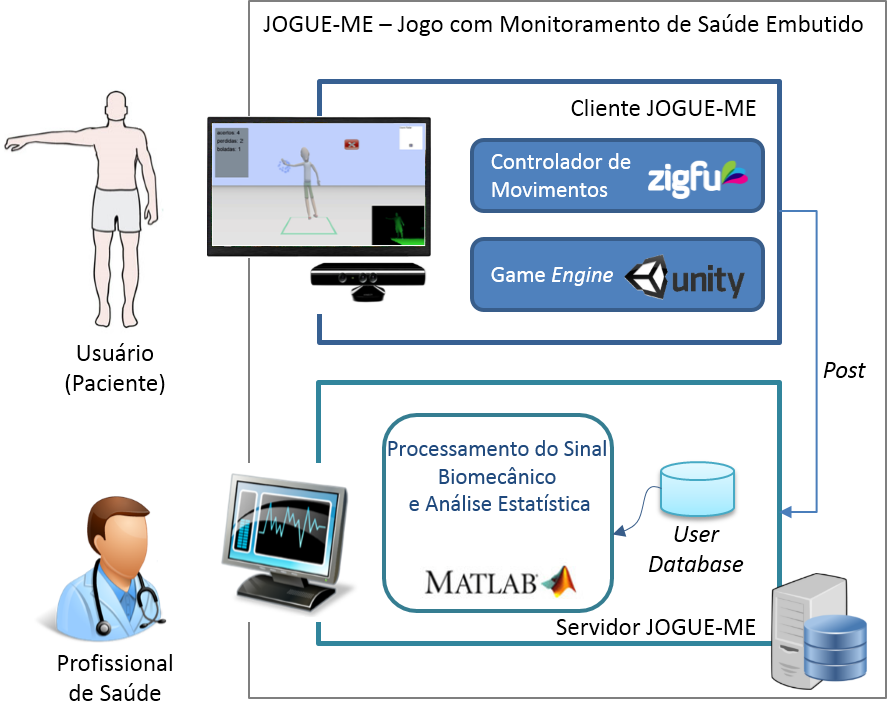
\includegraphics[width=0.78\textwidth]{./img/visaosistema.png}
     \caption{Visão Geral da Abordagem~\textit{JOGUE-ME}}
     \label{img:visaogeral}
\end{figure}
A abordagem~\ac{jogue-me} faz uso de jogos eletrônicos como interface de aquisição de sinais, tornando os usuários mais motivados a fornecer seus sinais motores, em comparação ao uso dos dispositivos vestíveis~\cite{alemdar}. Então, com o uso da presente abordagem, um paciente portador de uma doença motora, no conforto do seu lar, poderá fornecer sinais motores de uma maneira colaborativa e não invasiva. Por outro lado, o profissional de saúde poderá visualizar os sinais motores de seus pacientes com uma frequência muito maior, em comparação às avaliações clínicas realizadas durante o período de consulta. 

Nesse estudo, ao utilizar jogos eletrônicos como mecanismo para entrada de dados, é possível alcançar os requisitos de não invasividade propostos nesta tese, pois, através dos dispositivos de sensores de movimento usados nesses ambientes, é possível desenvolver um jogo que motive o usuário a executar ações específicas para permitir o monitoramento de sinais motores. A partir de uma interface com o usuário, que permite enviar os dados capturados a um servidor, e armazenar estes dados para o acompanhamento da saúde motora por parte do profissional de saúde.

Para esta solução, propõe-se usar técnicas de processamento de sinais para reconhecer os padrões de movimento e identificar os sinais motores (Figura~\ref{img:visaogeral}). Para tornar isso factível é necessário identificar ciclos de movimento, filtrá-los e extrair características deste movimento. Após a extração das características, os dados são repassados para máquinas de aprendizagem, as quais são responsáveis por classificar os dados, baseadas em evidências estatísticas. Caso a máquina identifique algum usuário com distúrbio motor, ela poderá notificar o profissional de saúde para que este visualize os dados e tenha um melhor suporte para a tomada de decisão em relação ao tratamento.

O funcionamento da abordagem pode ser descrito como uma composição de quatro passos: aquisição dos sinais por meio de sensores, processamento de sinais biomecânicos, classificação dos dados e visualização. Estes passos são detalhados nas seções seguintes.

\section{Aquisição dos Sinais Por Meio de Sensores}
O cliente \ac{jogue-me} é um jogo com funcionalidades de aquisição de dados motores de movimentos específicos. Logo, ele realiza a captura e o envio de dados para um servidor, que recebe requisições para efetuar o recebimento e o armazenamento das informações, o que torna possível armazenar o histórico do usuário para um acompanhamento dos sinais motores por um longo período. Com o uso do~\ac{jogue-me} é possível adquirir os movimentos do paciente para identificar a evolução dos sinais do~\ac{dp}, e consequentemente, quantificar sua saúde motora. 

Atualmente, a análise dos sintomas motores é feita de forma subjetiva pelo cuidador ou esporádica pelo neurologista quando o paciente está em atendimento clínico, visto que, atualmente não existem mecanismos disponíveis em larga escala que permitam quantificar os sintomas motores ou acompanhar o tratamento a distância. Este projeto pretende atender a esta demanda e auxiliar a prática dos profissionais de saúde melhorando a qualidade de vida dos pacientes com~\ac{dp}.

Um sensor de movimentos como o MS-Kinect~\cite{kinnect2013}, por exemplo, possui uma câmera infravermelho capaz de reconhecer os movimentos de todo o corpo humano e identificar as posições das articulações anatômicas~\cite{hamill1999bases}, para análise da cinemática do movimento humano~\cite{mcginnis2013biomechanics}. 

Para mensurar os movimentos do paciente, utilizamos diretrizes médicas para avaliação motora do~\ac{dp} como a UPDRS~\cite{updrs87}, a qual, permite diagnosticar e acompanhar o progresso da doença. Logo, os dados adquiridos pelos sensores podem ser mensurados com o processamento dos sinais e reconhecimento de padrões para identificar a ocorrência de sintomas motores. 

Desta maneira, a aquisição dos sinais motores e a quantificação do movimento de seus usuários permitirá uma participação mais precisa do profissional de saúde.



\section{Processamento de Dados Biomecânicos}\label{sec:processador_bio}
%Estou colocando aqui para ver uma melhor posição
\begin{figure}[!htb]
     \centering
     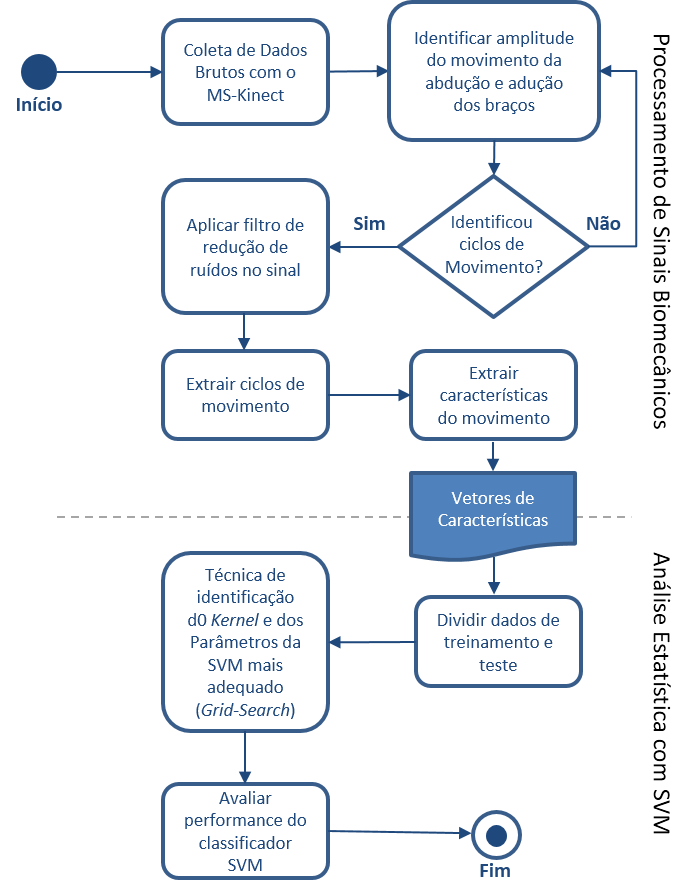
\includegraphics[width=0.8\textwidth]{./img/biomecprocessor2.png}
     \caption{Processamento de sinais biomecânicos.}
     \label{img:process_bio}
\end{figure}
O módulo de Processamento de Dados Biomecânicos é responsável por filtrar, remover ruídos e identificar ciclos de movimento para uma posterior extração dos vetores de características, como pode ser visto na Figura~\ref{img:process_bio}. A partir dos sinais processados, aplicam-se técnicas de aprendizagem de máquina para obter a classificação dos sinais e, consequentemente, validar este trabalho.




\subsection{Identificação de Ciclos de Movimento}\label{section:identificao_ciclos}

Os sinais adquiridos por sensores de movimento possuem bastante ruído, o que dificulta a identificação dos ciclos de movimento, pois eles possuem uma posição que inicia o ciclo de movimento, como na Figura~\ref{img:exsinalposicaopunho}, e o ruído existente pode cruzar por essa linha e consequentemente gerar falsas identificações. 

\begin{figure}[!htb]
     \centering
     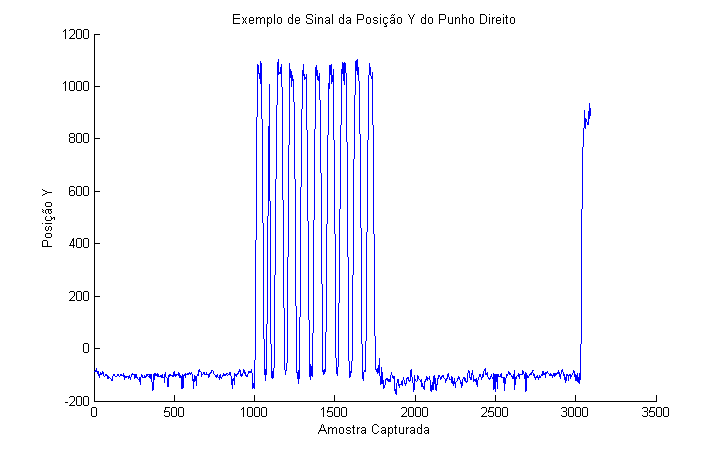
\includegraphics[width=1\textwidth]{./img/exsinalposicaoypunhodireito.png}
     \caption{Exemplo de Sinal Capturado da Articulação do Punho do Direito Usando MS-Kinnect na Posição Y}
     \label{img:exsinalposicaopunho}
\end{figure}


Em casos de análise de sinais biomecânicos da amplitude do movimento, é possível aplicar a técnica de detecção de picos e vales do sinal~\cite{peakdetect}. Esta técnica consiste em usar um valor de referência, $\delta$\ (\textit{delta}), para identificação dos picos, e descartar valores menores que são considerados ruídos. O pico é o ponto mais alto entre os 2 pontos mais baixos, que são considerados os vales do ciclo. A técnica é aplicada no sinal, com um $\delta$\ de 500, obtendo-se como resultado os picos e os vales identificados como pode ser visto na Figura~\ref{img:expicosvales}.

\begin{figure}[!htb]
     \centering
     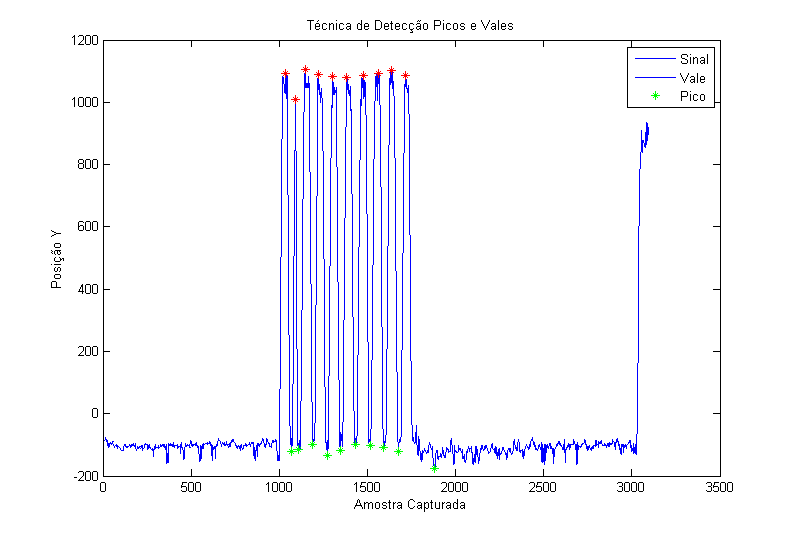
\includegraphics[width=1\textwidth]{./img/deteccaopicosvales.png}
     \caption{Exemplo da Aplicação da Técnica de Detecção de Picos e Vales no Sinal}
     \label{img:expicosvales}
\end{figure}


%\subsubsection{Redução de Ruídos no Sinal}
O processo de Identificação de Ciclos de Movimento é realizado em 3 etapas distintas:
\begin{itemize}
	\item identificar ciclos de movimentos;
	\item calcular movimento angular realizado durante o ciclo de movimento;
	\item remover ciclos de movimentos incompletos.
\end{itemize}

Para identificar os ciclos de movimento de adução e abdução dos braços, é necessário utilizar uma das articulações como referência. Neste movimento, a articulação do punho (Figura~\ref{img:exsinalposicaopunho}) é a que possui o sinal com maior amplitude entre as demais; por esse motivo, esta é a escolhida para identificar os ciclos. Realiza-se a técnica de picos e vales no sinal do \textit{punho} para identificar o início e o fim do movimento de adução e abdução dos braços. Depois de identificado onde começa e termina o movimento, calcula-se o deslocamento angular através do produto escalar entre as articulações do punho, do ombro e da bacia (Seção~\ref{section:movimento_abducao}). Neste momento, o sinal irá conter ciclos de movimentos angulares, então realiza-se uma nova eliminação de ruídos, ao extrair os ciclos de movimento identificados no sinal. Essa é a primeira etapa da filtragem dos dados, a qual seleciona o início e o fim dos ciclos de movimentos. Depois desta etapa, realiza-se a extração de cada ciclo e identifica-se sua completude, para que as características extraídas dos ciclos de movimento sejam semelhantes para cada indivíduo e torne possível a classificação dos dados.


%\begin{figure}[!htb]
     %\centering
     %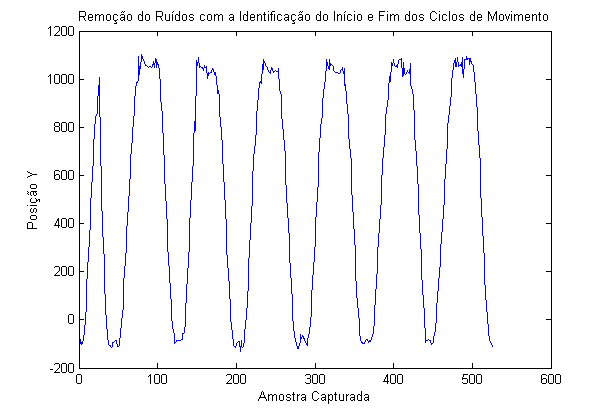
\includegraphics[width=1\textwidth]{./img/remocaoruidociclo.png}
     %\caption{Remoção de Ruídos}
     %\label{img:remocaoruidossinal}
%\end{figure}


\subsection{Extração das Características do Movimento} \label{sec:extracao_caracteristcas}
As características do sinal a ser obtido são baseadas na cinemática do movimento angular. Logo, é necessário um estudo da biomecânica do movimento humano nos ciclos de movimento~\cite{hamill1999bases}. De posse do tempo de ocorrência de cada ciclo e das articulações do \textbf{punho}, da \textbf{bacia} e do \textbf{ombro}, deve-se calcular o ângulo relativo do movimento de abdução e adução do braço através da aplicação do teorema do produto escalar, que encontra o ângulo entre dois vetores dentro do intervalo de $0 \leq \theta \leq 180º$.

\subsubsection{Cálculo do Ângulo Relativo do Movimento de Abdução e Adução}\label{section:movimento_abducao}
O produto escalar é uma operação entre dois vetores cujo resultado é um escalar~\cite{algebra2000}. Então, o ângulo entre dois vetores é definido como ``o menor'' ângulo entre eles. Dessa forma, este ângulo está dentro do intervalo de $0 \leq \theta \leq 180º $. O produto escalar é o ângulo de $ \theta$ formado entre os vetores $ v $ e $ w $.


% \begin{equation}
% cos(\theta) = (v . w) /  (||v|| ||w||) 
% \label{eq:produto_escalar}
% \end{equation}
% 
% 
% \begin{figure}[!htb]c
%      \centering
%      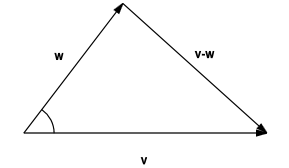
\includegraphics[width=0.5\textwidth]{./img/produtoescalar.png}
%      \caption{Produto Escalar Entre 2 Vetores}
%      \label{img:produto_escalar}
% \end{figure}

No movimento de abdução e adução do braço, o ângulo relativo pode ser calculado com as posições ($ x $\ ,  $ y $\ , $ z $\ ) das articulações (\textit{quadril}, \textit{ombro} e \textit{punho}). Utilizando o produto escalar entre esses pontos, extraem-se as características do movimento, como amplitude do movimento, e, quando relacionamos com o tempo, conseguimos extrair a velocidade angular deste movimento, como pode ser visto na Figura~\ref{img:amplitude_braco}, quantificando o movimento da adução e abdução do braço em relação ao tempo.


\begin{figure}[!htb]
     \centering
     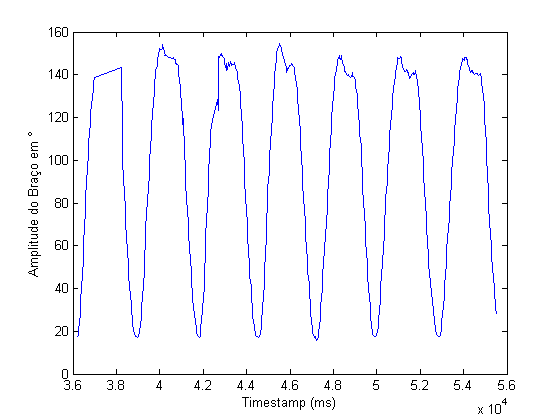
\includegraphics[width=1\textwidth]{./img/amplitude-braco.png}
     \caption{Amplitude do Movimento de Abdução e Adução}
     \label{img:amplitude_braco}
\end{figure}

\subsubsection{Cálculo da Velocidade Angular do Movimento de Abdução e Adução}
O pico da amplitude do movimento irá conter a amplitude máxima desse movimento. O tempo gasto entre o 1° vale e o pico em cada ciclo de movimento, será o tempo gasto para a abdução do braço, e o tempo gasto entre o pico e o 2° vale de cada ciclo, será o tempo gasto para a adução do braço. Portanto, com a amplitude máxima e o tempo gasto nesses movimentos, podem ser calculadas as velocidades angulares de abdução e adução dos braços, como pode ser visto na Figura~\ref{img:amplitude_braco_picos_vales}.
\begin{figure}[!htb]
     \centering
     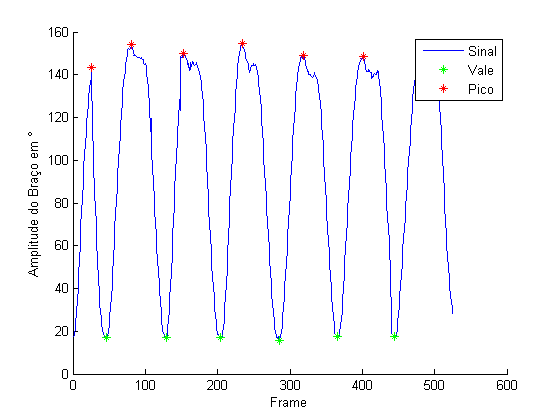
\includegraphics[width=1\textwidth]{./img/amplitude-braco-picos.png}
     \caption{Detecção de Picos e Vales da Amplitude do Movimento de Abdução e Adução do Braço}
     \label{img:amplitude_braco_picos_vales}
\end{figure}

\subsection{Filtragem de Dados}\label{section:filtro_dados}

A filtragem dos dados consiste na realização das seguintes etapas nos ciclos de movimento:
\begin{description}
	\item [Escalonamento dos ciclos]: O conjunto de dados deve possuir a distribuição de \textbf{M} amostras de vetores de dimensão \textbf{n}. Como os dados a serem analisados são sinais, deve-se então escalonar o sinal para uma dimensão \textbf{n} para poder realizar o cálculo matricial quadrático de (\textbf{M} x \textbf{n}).		
	\item [Normalização dos ciclos]: Em estatística, o termo normalização possui diferentes significados ~\cite{statisticterms2006}. Neste trabalho, a normalização consiste no ajuste dos valores dos dados em torno do valor máximo. Ou seja, o máximo valor obtido dos dados terá o valor 1, e os demais serão obtidos a partir da divisão do valor máximo. A normalização se faz necessária para que a variação dos dados seja mantida, além de facilitar a identificação de similaridades~\cite{vicini2005}. 	
	\item [Cálculo do Vetor Médio dos Ciclos]: Para definir a completude de um ciclo de movimento, deve-se calcular a média entre todos os ciclos de movimento, que é o vetor médio dos ciclos escalonados e normalizados. O \textbf{vetor médio}, Equação (\ref{eq:vetormedio}), chamado de $\bar{X}$, consiste na média aritmética de todos os ciclos de movimento, ou seja, ele define a centralização dos dados ~\cite{statisticshandbook2009}. 	
		\begin{equation}
			\bar{X}=\frac{\sum_{i=1}^{n}(Xi)}{(n)}
			\label{eq:vetormedio}
		\end{equation}
	\item [Calculo da Variância de Cada Ciclo ao Vetor Médio]: A variância é uma medida de dispersão estatística, que indica o quão longe os dados estão de um valor esperado~\cite{statisticshandbook2009}. Neste caso, o valor esperado é o vetor médio dos ciclos ($\bar{X}$), e a variância, Equação (~\ref{eq:variancia}), irá nos informar o quão distante cada ciclo ($C$) está em relação a média.
		\begin{equation}
			var(C) = (C - \bar{X} )^2
			\label{eq:variancia}
		\end{equation}
		
		
	\item [Definição do limiar para remoção de ciclos]: Essa etapa do processo de filtragem não é trivial, pois deve-se definir uma constante, $ filtro $\, que será comparada à variância do ciclo. Se esta for menor, será aceita; caso contrário, removida. Contudo, balancear entre o limiar de dispersão do ciclo de movimento e a média é complexo, pois existe uma grande variabilidade de movimento. Logo, um limiar muito alto pode acarretar na remoção de uma grande quantidade de ciclos. Por outro lado, um limiar baixo colocaria ruídos nos dados e, consequentemente, impactaria no resultado da classificação.	
	%\lstset{language=Matlab}
	%\begin{lstlisting}[frame=single, caption=Filtro dos Ciclos]  % Start your code-block
		%
    %filtro = 1;
    %vetorMedio = mean(ciclos);
    %varianciaCiclo = sum(ciclo - (vetorMedio).^2);
    %remocao = varianciaCiclo>filtro;
	%\end{lstlisting}
	%
\end{description}

	%\begin{figure}
     %\centering
     %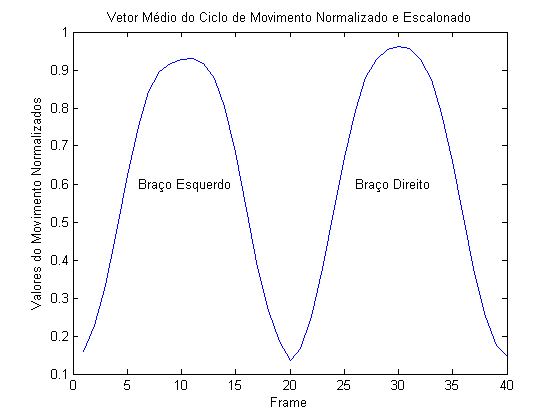
\includegraphics[width=1\textwidth]{./img/vetormedionormalozadoescalonado.png}
     %\caption{Ciclos de Movimento Normalizados e Escalonados}
		 %\label{img:ciclos_normalizado_escalonado}
	%\end{figure}

Como exemplo, temos um ciclo de movimento removido (Figura~\ref{img:ciclo_filtrado}), com \textit{valor do filtro = 1} e o \textit{valor da variância = 2,3078}.

\begin{figure}[!htb]
     \centering
     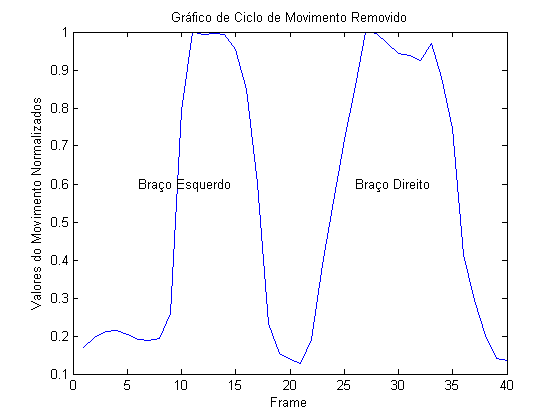
\includegraphics[width=1\textwidth]{./img/ciclomovimentoremovido.png}
     \caption{Ciclo de Movimento Removido}
		 \label{img:ciclo_filtrado}
\end{figure}


\section{Classificação de Dados por Máquina de Aprendizagem}\label{section:class_dados}
O objetivo de todo esse processo de identificação de ciclos, extração de características e filtragem é justamente facilitar a separação dos dados por máquinas de aprendizagem. A normalização dos ciclos ficou como o resultado do cálculo do produto escalar, que nos retorna valores entre $ 0° $\ a $ 180° $\, do movimento de abdução e adução. O escalonamento de cada ciclo de movimento ficou com 20 \textit{frames}. Como temos o movimento do braço esquerdo e depois o do direito, temos um total de 40 \textit{frames} por ciclo. O motivo pelo qual decidimos juntar os ciclos dos braços esquerdo e direito foi justamente para facilitar a identificação da assimetria do movimento existente nos estágios iniciais do~\ac{dp}. Portanto, o classificador será responsável por identificar os indivíduos diagnosticados com~\ac{dp}, por meio das diferenças de movimento existente entre estes e os indivíduos sem o diagnóstico da doença. 

O vetor de características é composto dos ciclos de movimento e das características extraídas de cada ciclo, conforme explicado na Seção~\ref{sec:extracao_caracteristcas}. Ou seja, terá, além do ciclo de movimento, os valores da velocidade angular de abdução e adução do braço esquerdo e direito. De posse desse vetor de características e do rótulo sobre a classe do ciclo de movimento (indivíduo diagnosticado com~\ac{dp} e indivíduo sem o diagnóstico estabelecido), esses dados serão repassados como entrada-saída para o classificador de dados, que irá dividir entre grupos de treinamento e teste para realizar sua classificação.

Nesta abordagem, o classificador de dados será usado para identificar usuários com problemas motores. Dessa forma, irá auxiliar o profissional de saúde no acompanhamento de seus pacientes. Supondo que um profissional de saúde detém um grande número de pacientes, e que estes fazem uso da abordagem~\ac{jogue-me} para monitorar seus dados, caso fosse identificada alguma anormalidade motora, o profissional de saúde seria notificado e poderia visualizar as informações que poderiam auxiliar na tomada de decisão.





\section{Visualização dos Dados}
O acompanhamento dos sinais motores é necessário, principalmente, para doenças crônicas de impacto motor e que tenham melhoria nos sinais, pois dessa maneira auxilia o médico no acompanhamento motor e, consequentemente, permite tratar o paciente de acordo com a resposta ao tratamento.

Como exemplo da abordagem, o profissional de saúde poderia visualizar as características dos movimentos, que serviram como dados de entrada para a máquina de aprendizagem. Nesse caso, podemos ver duas tabelas em que é possível identificar as diferenças motoras de uma pessoa diagnosticada com ~\ac{dp} (Tabela~\ref{table:extracao-caracteristica}) e um indivíduo sem o diagnóstico da doença (Tabela~\ref{table:extracao_caracterisca_saudavel}).

\begin{table}[h]
\begin{tabular}{|r|r|r|r|r|r|}
\hline
\multicolumn{4}{|l}{Velocidades º/S}                                                                                                                                                                                                                                                                                         & \multicolumn{2}{|l|}{Amplitudes}     \\ \hline
\multicolumn{1}{|l}{\textbf{\begin{tabular}[c]{@{}c@{}}Abdução\\ Esquerda\end{tabular}}} & \multicolumn{1}{|l|}{\textbf{\begin{tabular}[c]{@{}c@{}}Abdução\\ Direita\end{tabular}}} & \textbf{\begin{tabular}[c]{@{}c@{}}Adução\\ Esquerda\end{tabular}} & \textbf{\begin{tabular}[c]{@{}c@{}}Adução\\ Direita\end{tabular}} & \textbf{Esquerda} & \textbf{Direita} \\ \hline
78,95                                                                                    & 77,82                                                                                    & 83,06                                                              & 106,42                                                            & 130,00            & 124,72           \\ \hline
79,94                                                                                    & 34,68                                                                                    & 104,69                                                             & 39,98                                                             & 131,50            & 132,44           \\ \hline
81,05                                                                                    & 47,05                                                                                    & 107.38                                                             & 56,52                                                             & 132,22            & 123,66           \\ \hline
74,73                                                                                    & 47,09                                                                                    & 109,05                                                             & 47,75                                                             & 132,33            & 122,20           \\ \hline
72,01                                                                                    & 56,02                                                                                    & 102,36                                                             & 76,00                                                             & 131,40            & 119.75      \\ \hline
\end{tabular}
\caption{Extração das Características de Indivíduo Com Diagnóstico da ~\ac{dp}}
\label{table:extracao-caracteristica}
\end{table}

\begin{table}[h]
\begin{tabular}{|r|r|r|r|r|r|}
\hline
\multicolumn{4}{|l}{Velocidades º/S}                                                                                                                                                                                                                                                                                         & \multicolumn{2}{|l|}{Amplitudes}       \\ \hline
\multicolumn{1}{|l}{\textbf{\begin{tabular}[c]{@{}c@{}}Abdução\\ Esquerda\end{tabular}}} & \multicolumn{1}{|l|}{\textbf{\begin{tabular}[c]{@{}c@{}}Abdução\\ Direita\end{tabular}}} & \textbf{\begin{tabular}[c]{@{}c@{}}Adução\\ Esquerda\end{tabular}} & \textbf{\begin{tabular}[c]{@{}c@{}}Adução\\ Direita\end{tabular}} & \textbf{Esquerda} & \textbf{Amplitude} \\ \hline
129,35                                                                                   & 61,59                                                                                    & 78,74                                                              & 176,30                                                            & 159,39            & 143,50             \\ \hline
115,67                                                                                   & 118,15                                                                                   & 71,72                                                              & 79.46                                                             & 156,37            & 153,97             \\ \hline
120.96                                                                                   & 135,27                                                                                   & 66,70                                                              & 78,17                                                             & 154,30            & 149,91             \\ \hline
125.96                                                                                   & 137,43                                                                                   & 64,75                                                              & 81,57                                                             & 153,18            & 154,58             \\ \hline
139.99                                                                                   & 117,60                                                                                   & 69,96                                                              & 84,08                                                             & 151,68            & 148,90             \\ \hline
120,51                                                                                   & 111,92                                                                                   & 75,85                                                              & 75,18                                                             & 152,58            & 148,35             \\ \hline
\end{tabular}
\caption{Extração das Características de Indivíduo Sem Diagnóstico da ~\ac{dp}}
\label{table:extracao_caracterisca_saudavel}
\end{table}

Como pode ser visto nesses dados, a amplitude de um indivíduo diagnosticado com~\ac{dp} está bem menor do que em um indivíduo sem o diagnóstico estabelecido. Um valor importante também pode ser identificado na velocidade de adução esquerda do indivíduo com~\ac{dp}, pois este possui uma velocidade muito maior do que o indivíduo sem o diagnóstico. Possivelmente, porque um paciente com~\ac{dp} perde um pouco o controle sobre o membro, fazendo-o descer abruptamente~\cite{protpar010}. Dessa maneira, a abordagem pretende auxiliar o profissional de saúde com o fornecimento dessa informação, para que este efetue o acompanhamento e perceba a evolução do quadro clínico do paciente.

\section{Conclusão}
Neste capítulo, foram apresentados os requisitos que definiram a visão geral da abordagem~\ac{jogue-me}. Uma seção relevante deste capítulo é como será o processamento dos dados biomecânicos, nesta seção é demonstrada como será a extração de características a partir dos sinais adquiridos por sensores de movimento. Posteriormente, foi apresentada a importância da aprendizagem de máquina neste trabalho para identificar os usuários que possuem problemas motores.

Do ponto de vista clínico, foram citados os parâmetros cinemáticos quantificados que irá auxiliar o profissional de saúde na sua tomada de decisão. 

No capítulo seguinte, será apresentada a arquitetura de software que define a implementação da abordagem ~\ac{jogue-me}.